\documentclass[tikz]{standalone}
\usepackage{pgfplots}
\pgfplotsset{compat=1.15}
\usepackage{mathrsfs}
\usetikzlibrary{arrows,calc}
\usepackage{tkz-euclide}

\pagestyle{empty}

\definecolor{AngleClr}{rgb}{0,0.39215686274509803,0}
\definecolor{ShapeClr}{rgb}{0.6,0.2,0}
\definecolor{BlueClr}{RGB}{5,81,163}

\begin{document}

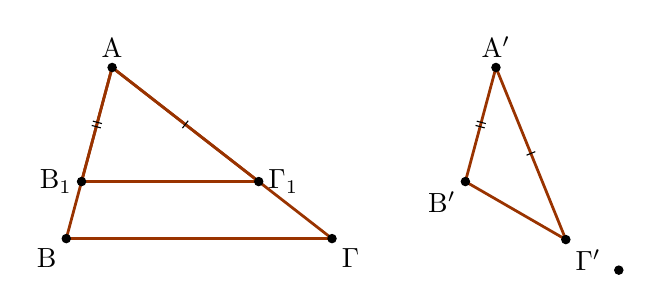
\begin{tikzpicture}[scale=.75]
\tkzSetUpLine[line width=1pt,color=black]
\tkzSetUpPoint[fill=black]

\tkzDefPoints{0/0/B,0/0/C1,6.5/0/C2}
\tkzDefShiftPoint[B](75:2){A}
\tkzDefShiftPoint[B](0:3){C}

\tkzDefPointOnLine[pos=1.5](A,B) \tkzGetPoint{B'}
\tkzDefPointOnLine[pos=1.5](A,C) \tkzGetPoint{C'}

\tkzFindAngle(C,B,A) \tkzGetAngle{aCBA}


\tkzDefPointsBy[translation=from C1 to C2](A,B){AA,BB}

\tkzCalcLength(A,C) \tkzGetLength{rAC} 
% 75 + (75 + x) = 180
\tkzDefShiftPoint[BB](-30:3){Cx}
\tkzInterLC[R](BB,Cx)(AA,\rAC) \tkzGetPoints{Y}{CC}



\tkzFillPolygon[fill=white](A,B,C)

\tkzFillPolygon[fill=white](AA,BB,CC)


\tkzDrawPolygon[color=ShapeClr](A,B,C)
\tkzDrawPolygon[color=ShapeClr](AA,BB,CC)
\tkzDrawPolygon[color=ShapeClr](A,B',C')

\tkzDrawPoints[size=3](A,B,C,AA,BB,CC,Cx,B',C')

\tkzLabelPoint[above](A){$\rm A$}
\tkzLabelPoint[left](B){$\rm B_1$}
\tkzLabelPoint[right](C){$\rm \Gamma_1$}
\tkzLabelPoint[below left](B'){$\rm B$}
\tkzLabelPoint[below right](C'){$\rm \Gamma$}


\tkzLabelPoint[above](AA){$\rm A'$}
\tkzLabelPoint[below left](BB){$\rm B'$}
\tkzLabelPoint[below right](CC){$\rm \Gamma'$}

\tkzMarkSegments[mark=||,size=1.7](A,B AA,BB)
\tkzMarkSegments[mark=|,size=1.7](A,C AA,CC)

\end{tikzpicture}

\end{document}
